\documentclass{article}
\usepackage{graphicx}
\usepackage{float}


\title{MakeFile for \LaTeX{}}
\date{\today}
\author{Eureka}
\begin{document}
\maketitle

\section{Puer makefile}
don't use \verb|latexmk| for autocompile, just 
use \verb|xelatex, pdflatex, lualatex|, which means 
that reference will be compile twice to show correctly.



\subsection{Why makefile}
To illustrated a situation you need to use make file,
there is an example:

{\itshape
    there is a picture in your file need to be compile first,
    after the picture is created, then you can compile your 
    .tex file to import the picture create just before.
}


There is only a file \verb|pic1.tex|, to include it in \verb|main.pdf|:
\begin{itemize}
    \item compile \verb|pic1.tex| to \verb|pic1.pdf|
    \item then compile \verb|main.tex| to import \verb|pic1.pdf|
\end{itemize}


\begin{figure}[H]
    \centering
    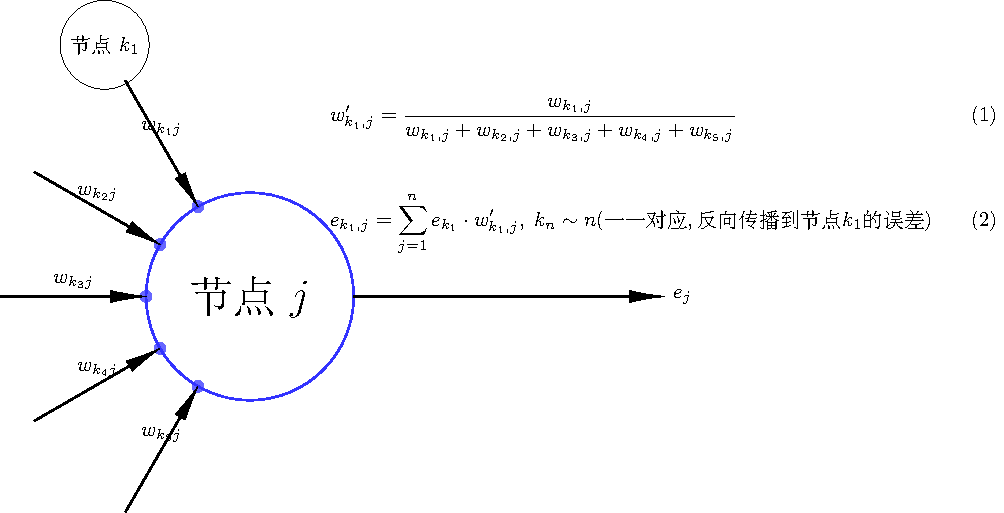
\includegraphics[width=.5\linewidth]{./Pic1.pdf}
\end{figure}

\textbf{Addtionally}: tool \verb|make| will check if your file 
has changed, if so it will recompile it, if not, this file will 
remain unchanged, which means: you can archieve people's "part compile"
to speed up!



\section{makefile \& latexmk}
\subsection{latexmk install}
go to CTAN \verb|https://www.ctan.org/pkg/latexmk/|, downloading 
source file, see file \verb|INSTALL| to install \verb|latexmk|
on your system.


\subsection{use latexmk with makefile}
\verb|latexmk| to make your compile more fluent, but to my 
own prescription: \verb|latexmk| is a burden, when you grab 
the compile process of \TeX{}.

to make this article more compatible, i will ref several point 
when using \LaTeX{}MK. 




\end{document}
